\documentclass[11pt]{article}

\usepackage[letterpaper,margin=1in]{geometry}
\usepackage[T1]{fontenc}
\usepackage[utf8]{inputenc}
\usepackage{lmodern}
\usepackage{microtype}
\usepackage{graphicx}
\usepackage{booktabs}
\usepackage{longtable}
\usepackage{tabularx}
\usepackage{array}
\usepackage{enumitem}
\usepackage{amsmath}
\usepackage{xspace}
\usepackage{xcolor}
\usepackage{hyperref}
\usepackage{xurl}
\usepackage{url}

\graphicspath{{figures/}}
\hypersetup{
  colorlinks=true,
  linkcolor=blue!45!black,
  citecolor=blue!45!black,
  urlcolor=blue!45!black
}

\newcommand{\sys}{Evanesca\xspace}
\newcommand{\numtransactions}{14,187,803\xspace}
\newcommand{\numincidents}{40\xspace}
\newcommand{\numflagged}{1,418\xspace}
\newcommand{\numbaseline}{956\xspace}
\newcommand{\numnonbaseline}{462\xspace}
\newcommand{\numreward}{207\xspace}
\newcommand{\numprice}{166\xspace}
\newcommand{\numyield}{12\xspace}
\newcommand{\numother}{77\xspace}
\newcommand{\numdefects}{219\xspace}
\newcommand{\numconstraints}{nine\xspace}
\newcommand{\constraint}[1]{{\footnotesize\texttt{#1}}}
\emergencystretch=2em

\title{\sys Technical Report:\\
Open-Source Forensic Reconstruction of DeFi Value Extraction}
\author{Evanesca Project}
\date{Public-release draft, July 2026}

\begin{document}
\maketitle

\begin{abstract}
\sys is an open-source framework for reconstructing decentralized-finance
(DeFi) transactions as Semantic Financial Graphs (SFGs) and auditing those
graphs with transparent financial constraints. This report reorganizes the
paper-era \sys research prototype as a public technical report and release
document. The emphasis is forensic reconstruction, measurement, and
analyst-facing evidence export, not real-time exploit detection or automatic
attribution of malicious intent. We describe the threat model, financial
semantics, SFG abstraction, constraint methodology, case-study evidence,
paper-era measurement results, public artifacts, and remaining limitations.
The current release includes source code, documentation, a JSON evidence
schema, a replayed bZx case-study artifact, and public hash-set manifests.
\end{abstract}

\section{Positioning}
\sys should be read as a measurement and forensic reconstruction framework.
It does not claim to be a production exploit detector, a low-false-positive
monitor, or a system that infers malicious intent from traces alone. Its output
is a candidate event: a transaction-local evidence trace that satisfies one or
more financial constraints and therefore deserves analyst review.

This framing is important because value extraction in DeFi spans routine market
activity and harmful protocol abuse. MEV and arbitrage can move value without a
software defect~\cite{flashbots,weintraub2022flash,mevdef}, while flash-loan
and oracle incidents can use similar swap, borrow, and repay primitives to
extract value from a protocol-local economic assumption~\cite{qin2021attacking,zhou2023sok}.
\sys therefore separates reconstruction from final judgment:
\begin{itemize}[leftmargin=*]
  \item \textbf{candidate event}: a constraint-backed transaction or trace;
  \item \textbf{benign arbitrage}: value extraction that resolves price gaps
        without violating a protocol-local accounting, oracle, collateral,
        reward, bridge, or derivative-pricing rule;
  \item \textbf{harmful extraction}: abnormal value transfer caused by
        exploiting or violating such a protocol-local economic rule;
  \item \textbf{confirmed incident}: a publicly documented event with
        replayable on-chain transaction evidence and an external narrative.
\end{itemize}

The public release goal is narrower than a new conference submission. It is to
make the system, evidence format, and reproducibility path inspectable: source
code, technical report, documentation, reproducible artifacts, and example
datasets should agree with each other and should avoid unsupported claims.

\section{Motivation}
DeFi attacks are often presented as isolated incidents, but many share recurring
financial structure. A bZx-style price manipulation, a reward-distribution
abuse, and a derivative exchange-rate defect may involve different contracts
and event schemas, yet each can be inspected as an ordered sequence of financial
actions with value flow, pricing dependencies, and accounting relations.

Existing systems address important parts of this problem. DeFiRanger and
BlockEye focus on detecting known price-manipulation or attack patterns
\cite{wu2021defiranger,wang2021blockeye}. DeFort and DeFiScope further analyze
price manipulation with specialized logic~\cite{defort2024,zhong2025defiscope}.
Operational systems such as Forta and OpenZeppelin Defender provide
deployment-facing monitoring and alerting~\cite{forta2023whitepaper,ozdefender}.
These approaches are useful, but they tend to bind the analysis to a template,
deployment rule, or specific attack class. \sys instead starts from the
measurement question: what financial actions occurred, which service-class
assumptions were stressed, and how did value move?

\section{Threat Model}
\subsection{Adversary and Capabilities}
\sys models transactions created by ordinary users, arbitrageurs, liquidators,
MEV searchers, flash-loan users, and attackers. The sender may interact through
one or more externally owned accounts or contracts. An adversarial transaction
may compose multiple DeFi services atomically, borrow temporary capital, distort
an AMM, oracle, lending market, reward pool, bridge, or derivative price, and
then return most intermediate state to normal while retaining value.

The framework does not require private mempool access, block-builder control,
or sandwich capability as core assumptions. Such behavior can be represented
when visible in traces, but the core abstraction is transaction-local financial
reconstruction.

\subsection{Loss Subjects}
The affected party depends on the service class. \sys distinguishes protocol
reserves, liquidity providers, lending depositors, reward-pool participants,
derivative-token holders, bridge backing reserves, traders receiving worse
execution, and cases with no direct victim beyond market-efficiency arbitrage.
This distinction prevents the system from treating every profitable trade as a
harmful incident.

\section{System Overview}
Figure~\ref{fig:pipeline} shows the paper-era pipeline reused by the public
release. The report reuses figures from the IMC, DeFi 26, and arXiv-era
Evanesca drafts where they explain architecture or examples; empirical result
tables in this report use the IMC measurement snapshot unless explicitly marked
as validation evidence. The system has four stages.

\begin{figure}[t]
  \centering
  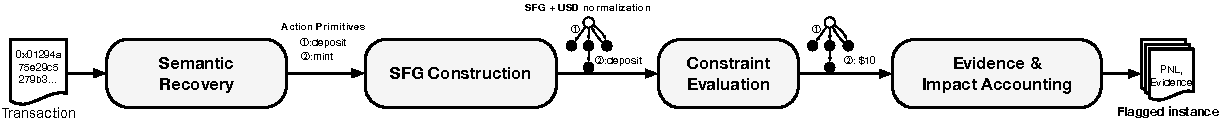
\includegraphics[width=\linewidth]{new_overview.pdf}
  \caption{\sys pipeline: semantic recovery, SFG construction, constraint
  evaluation, and evidence export.}
  \label{fig:pipeline}
\end{figure}

\paragraph{Semantic recovery.}
Protocol-specific adapters decode traces and event logs into typed financial
actions such as swap, deposit, withdraw, borrow, repay, liquidate, bridge, and
reward. The adapter boundary is deliberate: protocol-specific decoding belongs
in semantic recovery, while constraints should operate over service-class
financial actions rather than incident-specific signatures.

\begin{figure}[t]
  \centering
  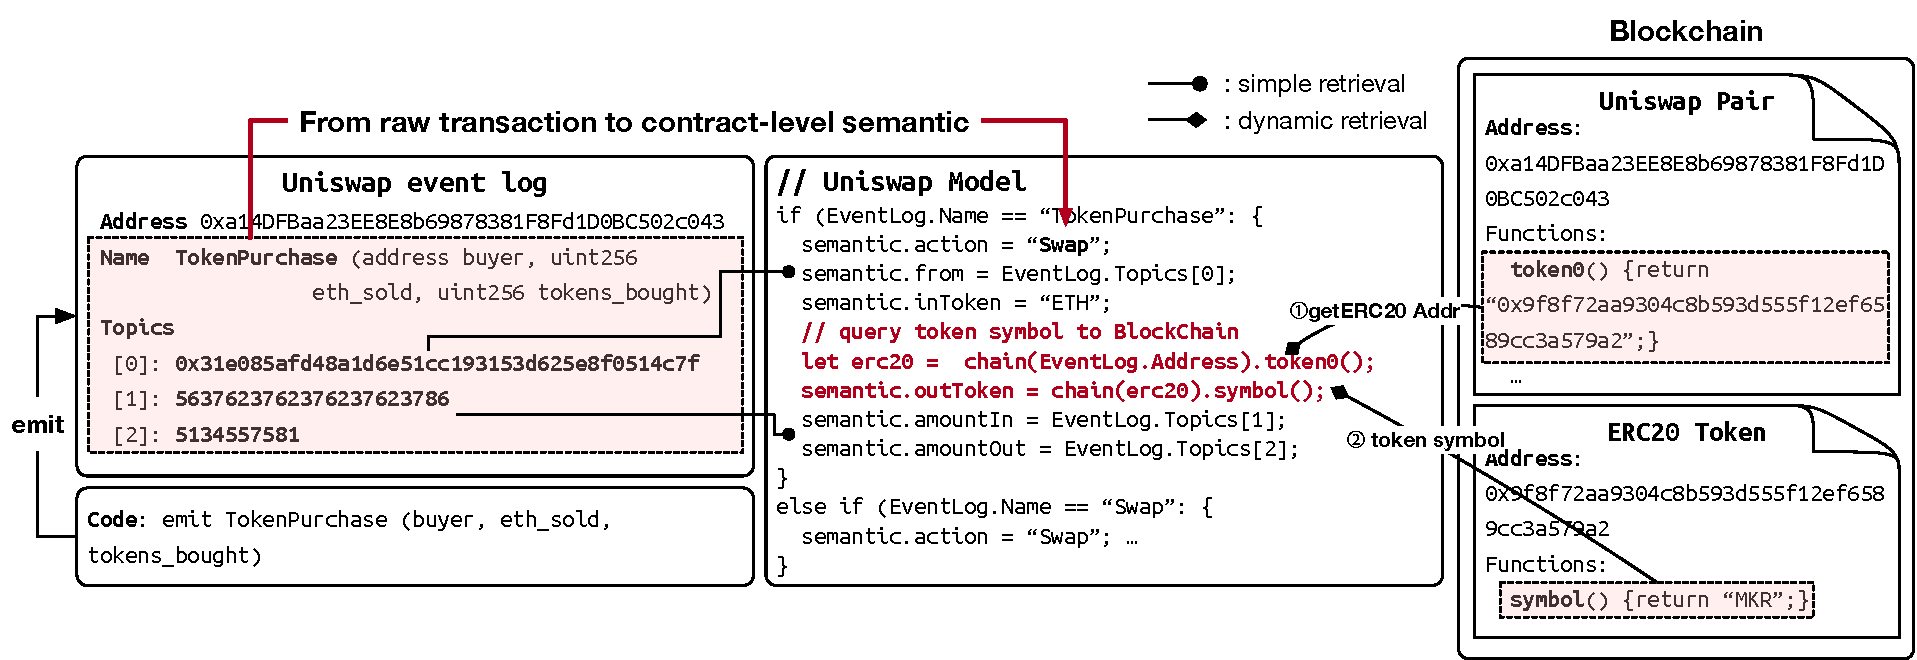
\includegraphics[width=\linewidth]{semantic_model.pdf}
  \caption{Semantic action model reused from paper-era Evanesca drafts. The
  figure documents the adapter boundary rather than adding a new experimental
  result.}
  \label{fig:semantic_model}
\end{figure}

\paragraph{SFG construction.}
Recovered actions are assembled into a directed graph \(G=(V,E)\). Vertices
represent accounts, contracts, pools, markets, services, and tokens. Edges
represent typed financial actions and carry token amounts, USD-normalized
values, protocol context, ordering, and raw evidence pointers. Raw transfers
alone are not enough because many DeFi incidents depend on shares, collateral,
debt, rewards, or derivative exchange rates that are not visible as a simple
token-transfer chain.

\paragraph{Constraint evaluation.}
Constraints encode service-class financial assumptions: AMM value consistency,
collateral sufficiency, oracle sanity, exchange-rate stability, reward
allocation fairness, flash-loan structure, and bridge backing. A match is a
candidate event, not an exploit verdict.

\paragraph{Evidence export.}
The public CLI exports JSON containing the transaction identity, summary,
graph, constraints, evidence timeline, and diagnostics. The current schema is
documented in \path{docs/public-api/analysis-result.schema.md}; example
outputs live under \path{docs/example-datasets/}.

\section{Semantic Financial Graph}
The SFG abstraction is not claimed as a novel graph data structure by itself.
Its contribution is the combination of reusable financial semantics, ordered
evidence export, and constraint evaluation over cross-protocol actions.

\begin{table}[t]
\centering
\caption{SFG elements exposed in the public evidence format.}
\label{tab:sfg}
\begin{tabularx}{\linewidth}{lX}
\toprule
Element & Public meaning \\
\midrule
Node & Account, protocol contract, pool, market, token, or service entity. \\
Edge & Typed financial action such as swap, borrow, repay, deposit, or transfer. \\
Value fields & Token amount, token symbol/address when known, and USD-normalized value. \\
Ordering & Transaction-local sequence used for evidence reconstruction. \\
Diagnostics & Unsupported actions, missing metadata, and recovery caveats. \\
\bottomrule
\end{tabularx}
\end{table}

Compared with cash-flow-only representations, \sys attempts to preserve
financial relations that matter for DeFi analysis: pricing dependencies,
collateral and debt relations, reward entitlement, derivative exchange-rate
relations, bridge mint/redeem backing, action ordering, and PnL attribution.

\begin{figure}[t]
  \centering
  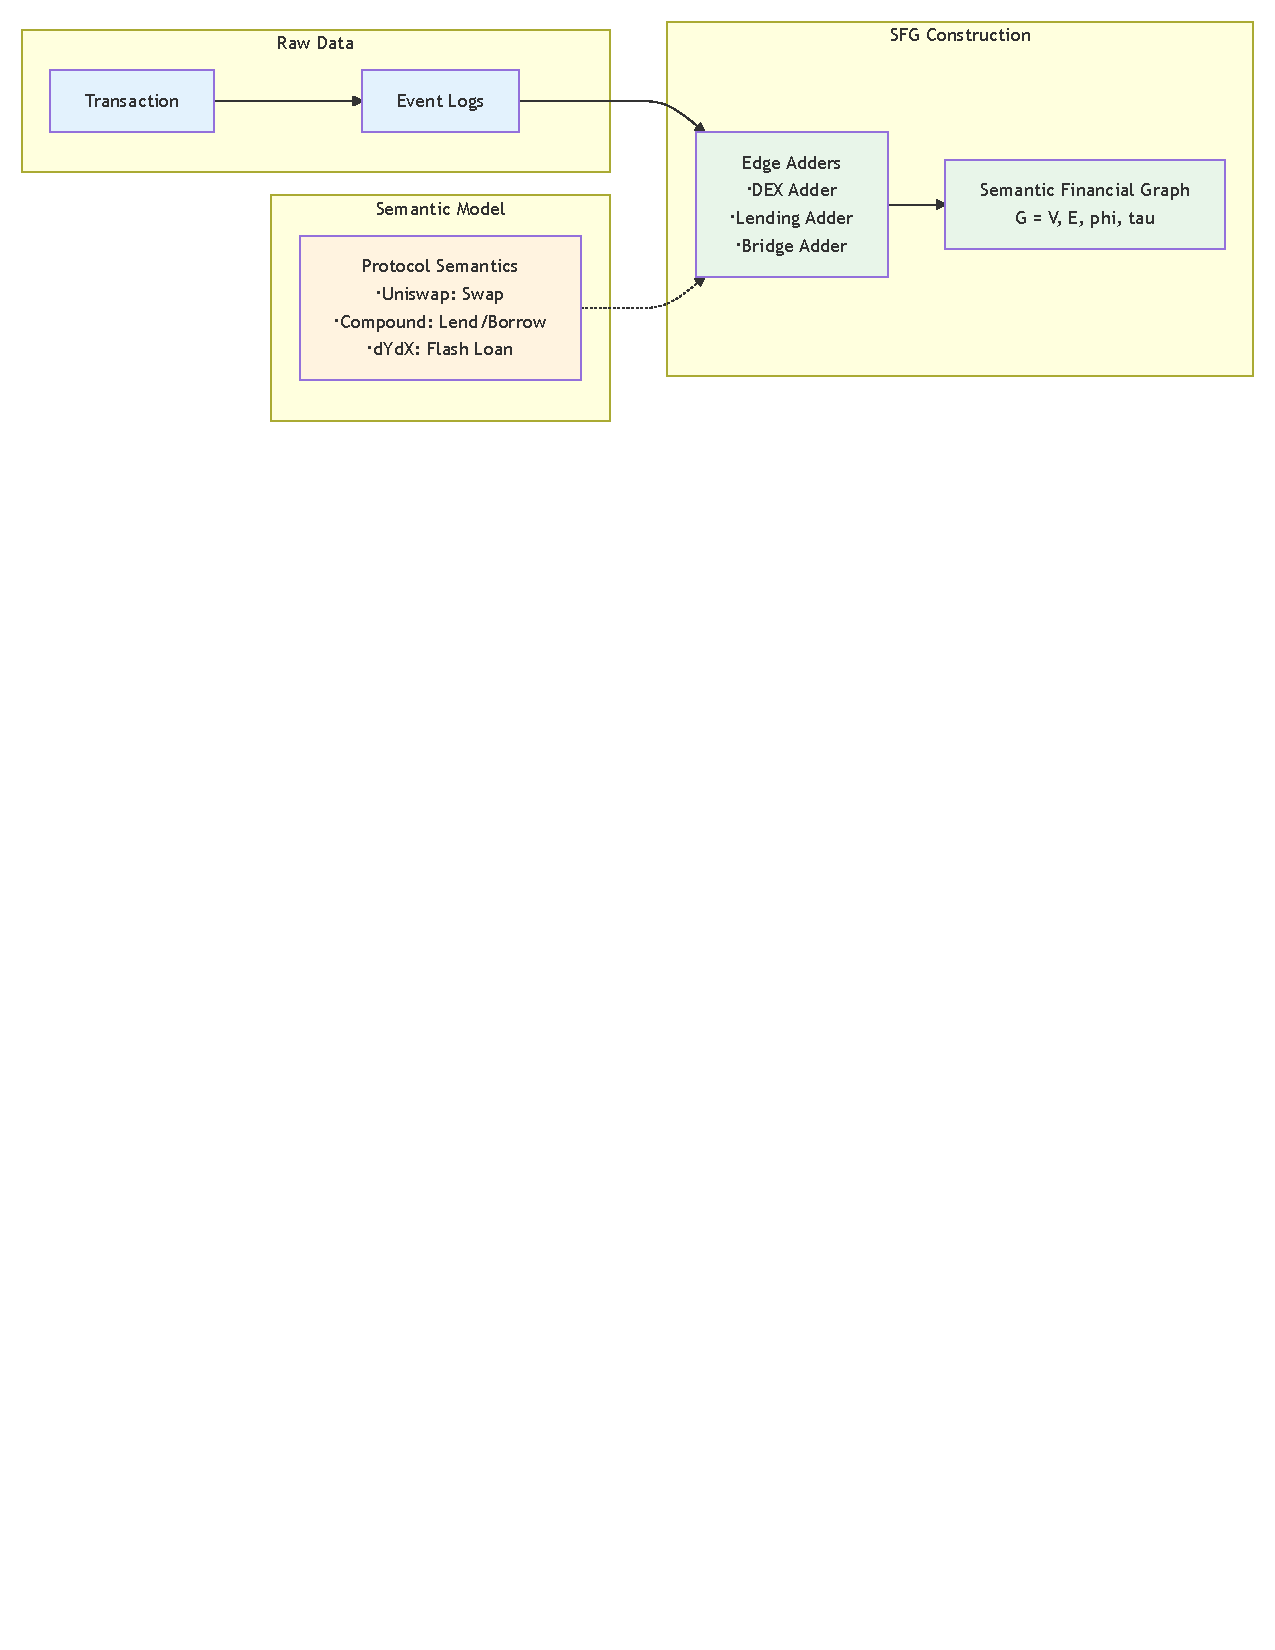
\includegraphics[width=\linewidth]{sfg-construction.pdf}
  \caption{SFG construction figure reused from paper-era Evanesca versions.}
  \label{fig:sfg_construction}
\end{figure}

\begin{figure}[t]
  \centering
  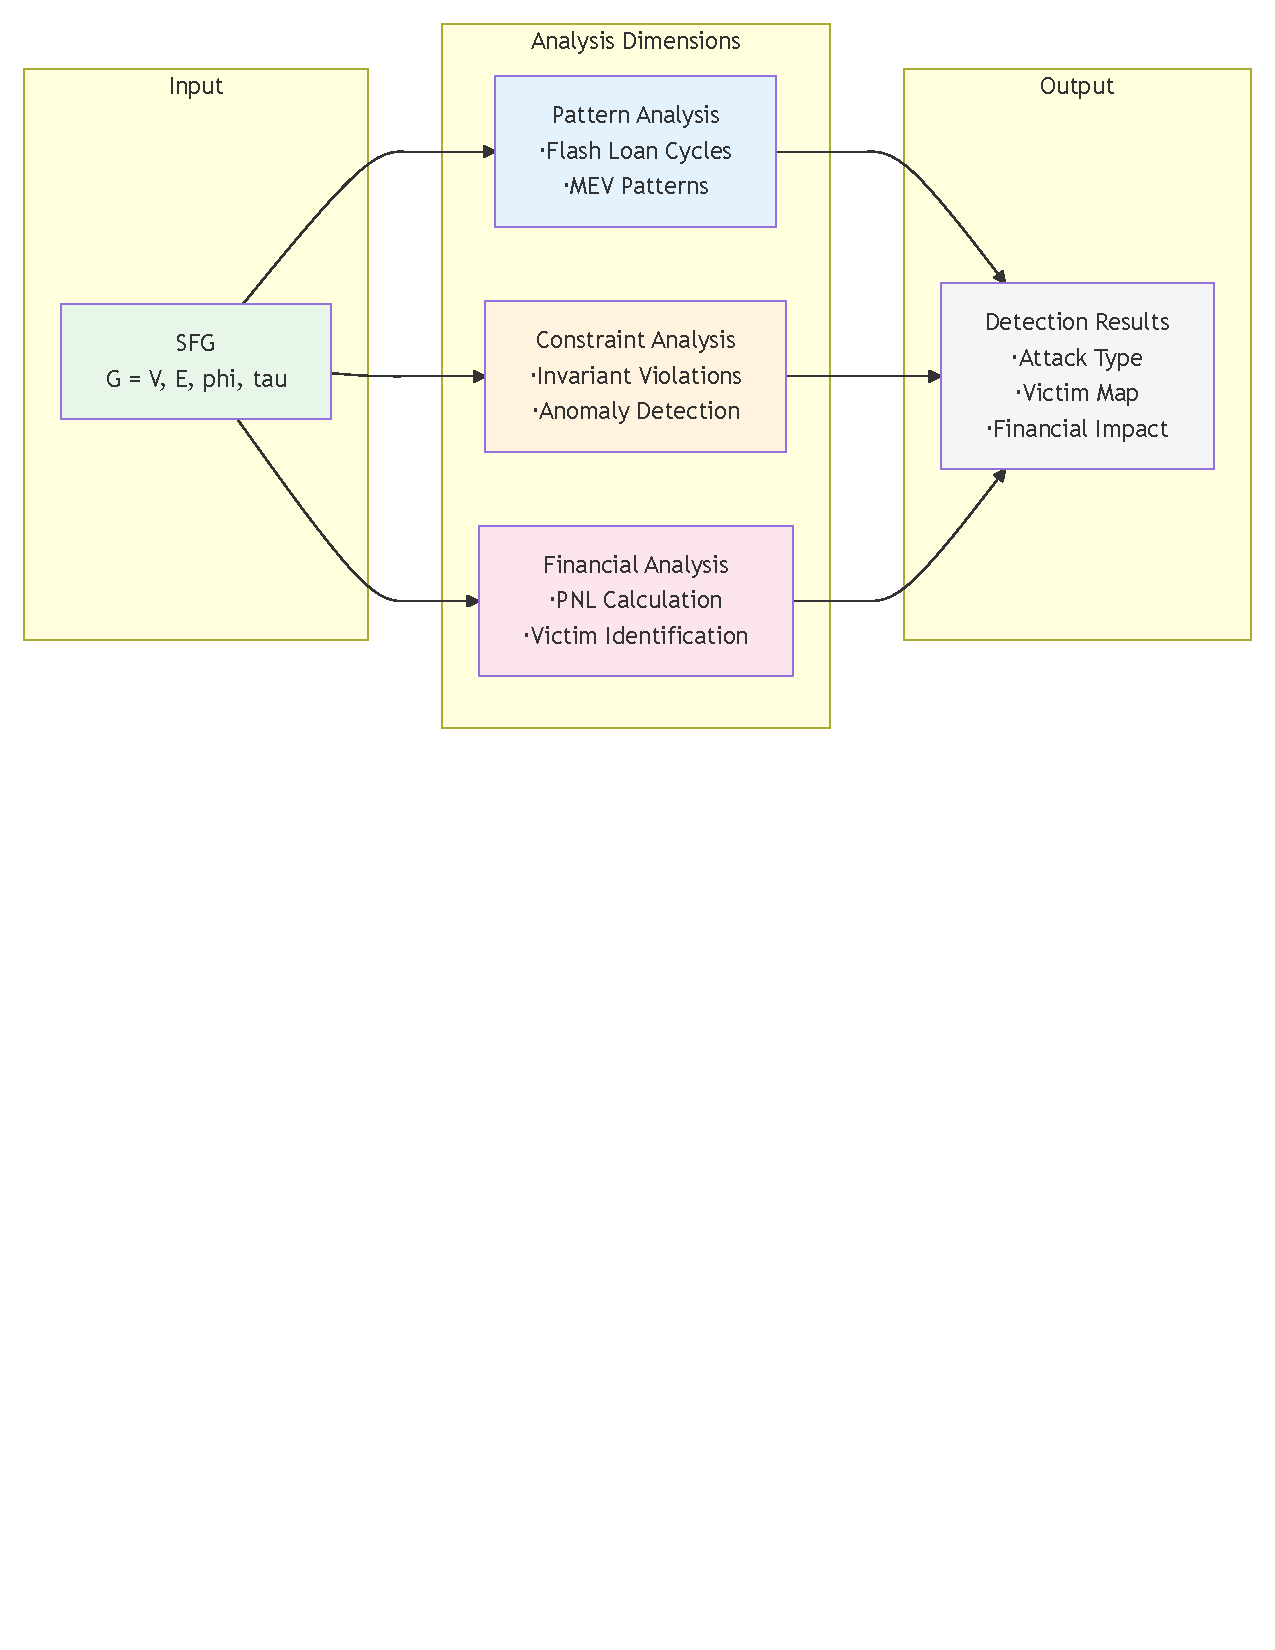
\includegraphics[width=\linewidth]{sfg-evaluation.pdf}
  \caption{SFG evaluation figure reused to explain how graph evidence feeds
  constraint checks.}
  \label{fig:sfg_evaluation}
\end{figure}

\section{Constraint Methodology}
For an edge \(e\) with nonzero USD input value, \sys commonly computes:
\[
  \rho(e) = \frac{\mathrm{valueUSD}(\mathrm{out}(e))}
                 {\mathrm{valueUSD}(\mathrm{in}(e))}.
\]
The paper-era implementation used \(\alpha=0.05\) for DEX swap edges and
\(\beta=0.02\) for lending or oracle-mediated stablecoin-derivative edges. The
DEX threshold is above reported routine unexpected slippage on Uniswap
\cite{zhou2021high}; the stablecoin-derivative threshold is tighter because
oracle studies report smaller normal movements for major stable assets
\cite{liu2021firstlook}. These thresholds are measurement parameters, not
universal constants. A release-quality benchmark still needs sensitivity
analysis and a public labeling protocol before making strong false-positive or
false-negative claims.

\begin{longtable}{p{0.31\linewidth}p{0.59\linewidth}}
\caption{Current paper-era constraint families.}\label{tab:constraints}\\
\toprule
Constraint family & Service-class signal \\
\midrule
\endfirsthead
\toprule
Constraint family & Service-class signal \\
\midrule
\endhead
\constraint{PRICE\_MANIPULATION} & Abnormal swap value ratio or price deviation. \\
\constraint{DEX\_K\_INVARIANT} & AMM reserve-invariant deviation or significant swap imbalance. \\
\constraint{LENDING\_COLLATERALIZATION} & Borrow, withdraw, or accounting behavior inconsistent with collateral assumptions. \\
\constraint{EXCHANGE\_RATE\_MANIPULATION} & Vault or derivative exchange-rate anomaly. \\
\constraint{ORACLE\_MANIPULATION} & Oracle-mediated price/accounting inconsistency. \\
\constraint{BRIDGE\_INTEGRITY\_VIOLATION} & Bridge backing or mint/redeem inconsistency. \\
\constraint{FLASH\_LOAN\_ATTACK} & Atomic temporary-capital pattern coupled with profit or manipulated state. \\
\constraint{CONCENTRATED\_LIQUIDITY\_ATTACK} & Tick, liquidity, or price-impact anomaly in concentrated-liquidity markets. \\
\constraint{EMPTY\_MARKET\_ATTACK} & Low-liquidity lending-market share-price anomaly. \\
\bottomrule
\end{longtable}

\begin{figure}[t]
  \centering
  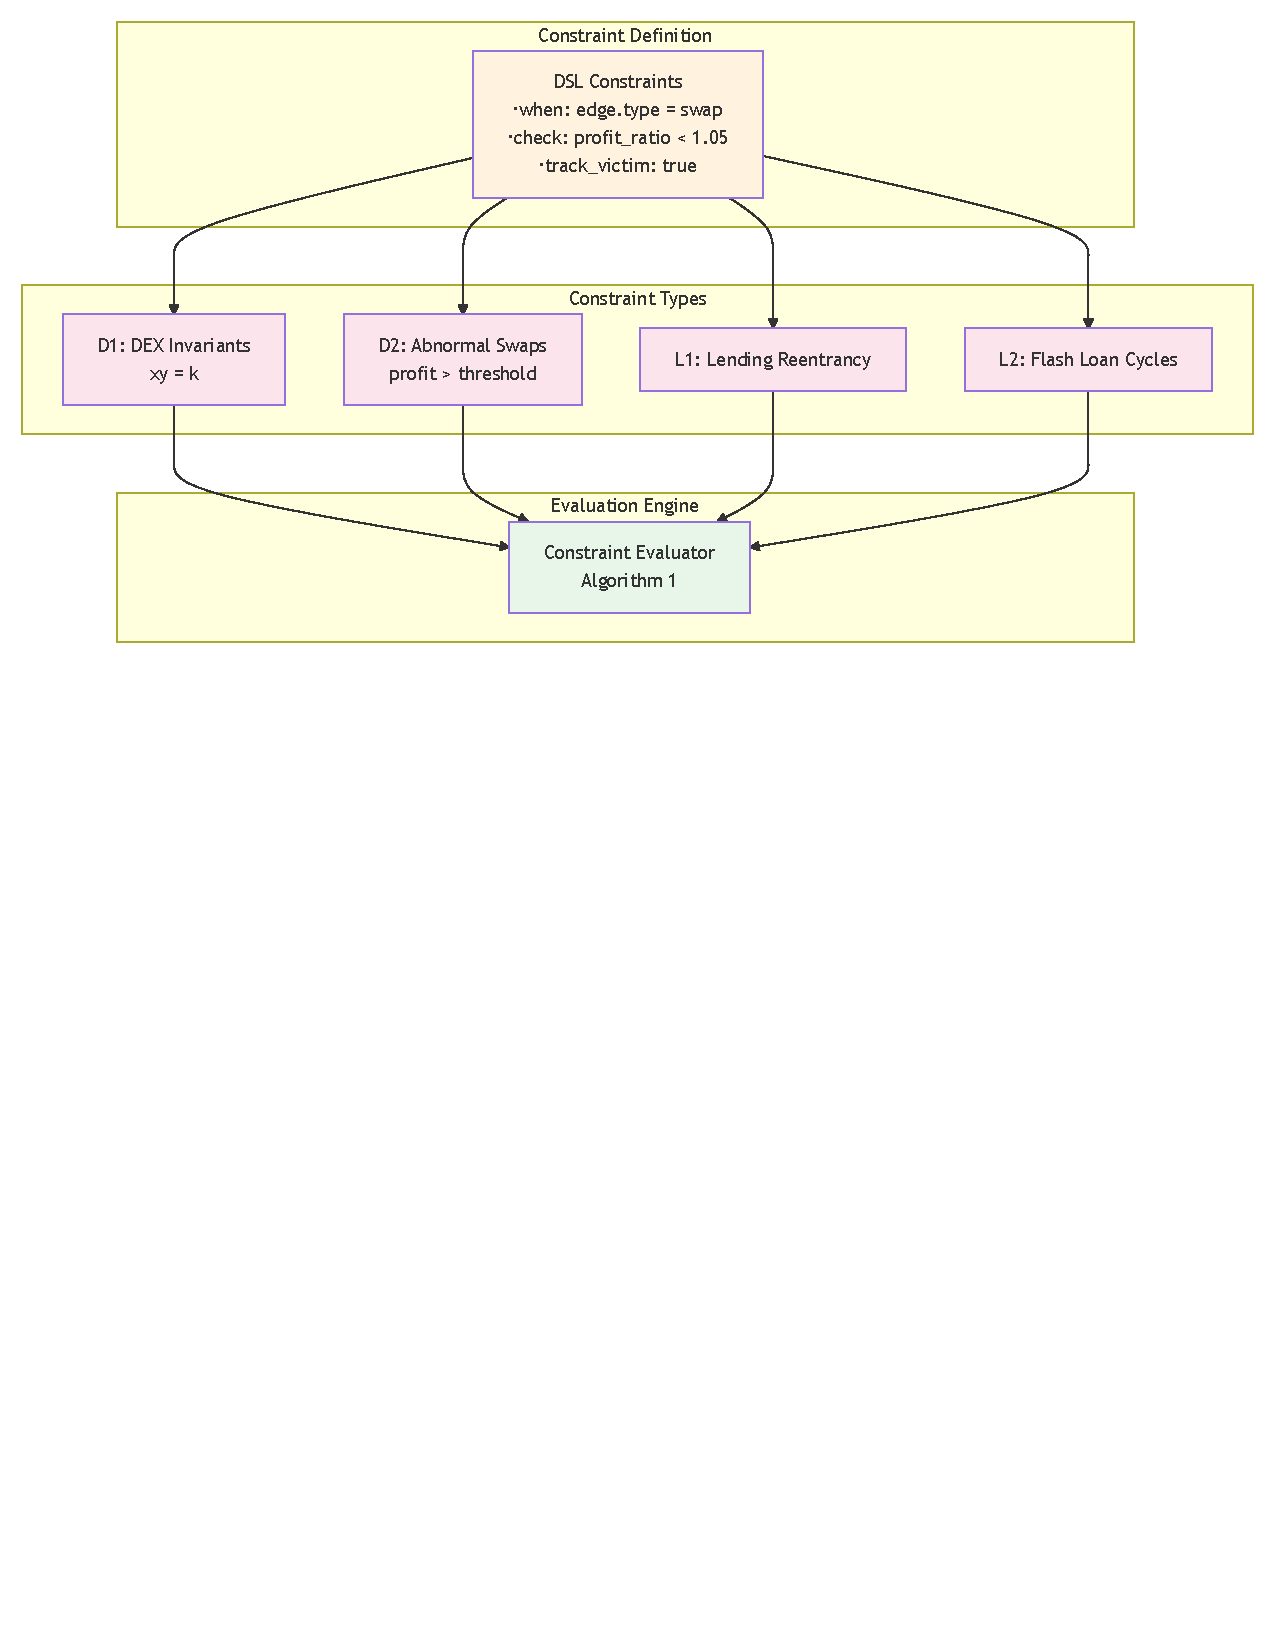
\includegraphics[width=\linewidth]{dsl-constraints.pdf}
  \caption{DSL constraint overview from the paper-era report. It is included as
  method documentation; the numeric evaluation below remains the IMC snapshot.}
  \label{fig:dsl_constraints}
\end{figure}

\section{Case Study: bZx Replay}
The public release currently includes one replayed case-study artifact:
\path{docs/example-datasets/bzx-analysis-result.json}. It is generated by:
\begin{verbatim}
npm run analyze -- --tx \
0xb5c8bd9430b6cc87a0e2fe110ece6bf527fa4f170a4bc8cd032f768fc5219838 \
--chain ethereum --out docs/example-datasets/bzx-analysis-result.json --pretty
\end{verbatim}

Figure~\ref{fig:bzx} shows the paper-era bZx walkthrough used to motivate the
pipeline. In the current public JSON export, the replayed transaction produces
10 graph nodes, 8 graph edges, 4 constraint records, and 8 evidence steps. The
summary status is \texttt{flagged}; the current classifier leaves the category
as \texttt{unattributed}. This is acceptable for a public schema example, but it
also makes clear that the open-source release should not overstate the current
classifier as a finished incident-labeling system.

\begin{figure}[t]
  \centering
  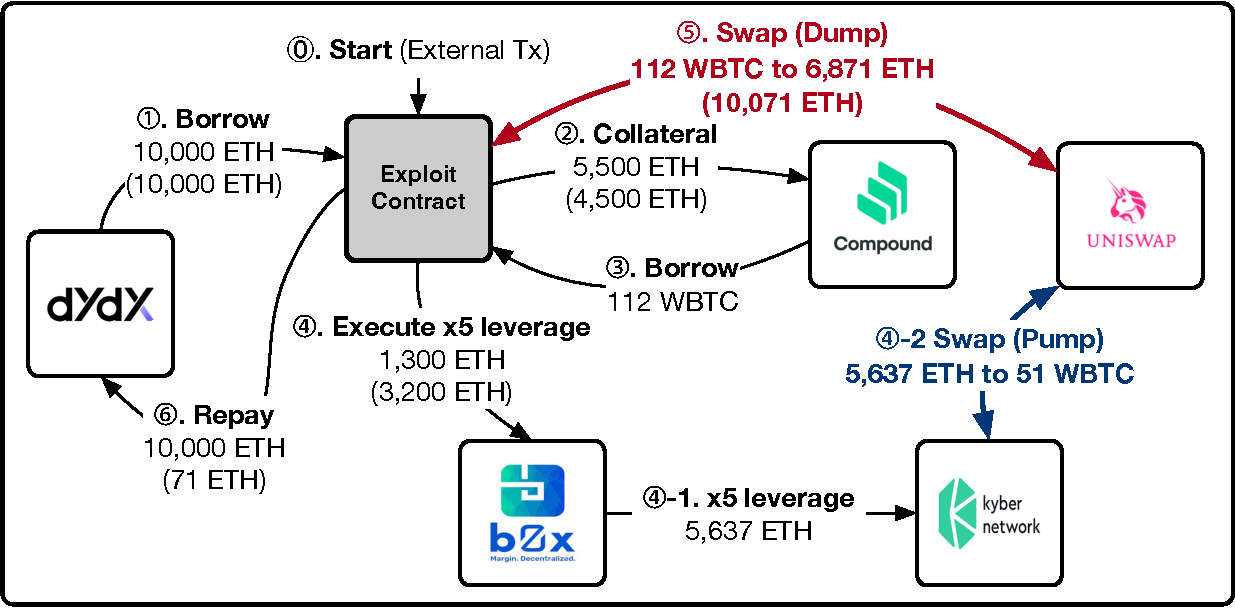
\includegraphics[width=\linewidth]{runningExample.pdf}
  \caption{Representative bZx-style price-manipulation pattern from the
  paper-era walkthrough.}
  \label{fig:bzx}
\end{figure}

\section{IMC Measurement Snapshot}
The following numbers summarize the IMC-version measurement snapshot. Other
paper-era drafts are useful for figures and validation context, but this report
does not import non-IMC scale-out result tables because some earlier drafts used
broader claims that still need revalidation. Public materials must present
these IMC numbers with scope qualifiers until the matching dataset manifests,
population reproduction commands, and labeling protocol are complete.

\begin{table}[t]
\centering
\caption{IMC scalar claims tracked for the public release.}
\label{tab:keynumbers}
\begin{tabularx}{\linewidth}{l>{\raggedleft\arraybackslash}p{0.22\linewidth}X}
\toprule
Quantity & Value & Public interpretation \\
\midrule
Ethereum transactions analyzed & \numtransactions & Research snapshot over supported DeFi interactions. \\
Confirmed incidents & \numincidents & Curated replay set requiring explicit inclusion/exclusion criteria. \\
Total flagged instances & \numflagged & Constraint-backed candidate events. \\
Baseline arbitrage & \numbaseline & Benign baseline, not harmful by default. \\
Non-baseline instances & \numnonbaseline & Candidates requiring category-level review. \\
Implementation-defect instances & \numdefects & Reward-distribution plus derivative-pricing families. \\
\bottomrule
\end{tabularx}
\end{table}

The non-baseline breakdown is: \numreward reward-distribution manipulation
instances, \numprice price-manipulation instances, \numyield yield-bearing token
deviation instances, and \numother unattributed long-tail candidates. The
public report intentionally separates these from the \numbaseline routine
arbitrage baseline. Treating the baseline as false positives would misstate the
measurement goal; treating all candidates as harmful would also be wrong.

\subsection{IMC Case-Study Partition}
The case-study partition follows the IMC version. Routine DEX arbitrage is
reported as a benign baseline when the trace shows cross-market convergence
without flash-loan, oracle, lending, reward, or derivative-pricing evidence. A
candidate becomes non-baseline when the same value-ratio signal is coupled with
state manipulation or cross-protocol dependency: price pumping, oracle-sensitive
borrowing, reward trigger timing, or yield-token deposit/withdraw conversion.
This distinction is why Figure~\ref{fig:patterns} is central to the public
report: it explains how \sys separates routine arbitrage from candidates that
need deeper review.

\begin{figure}[t]
  \centering
  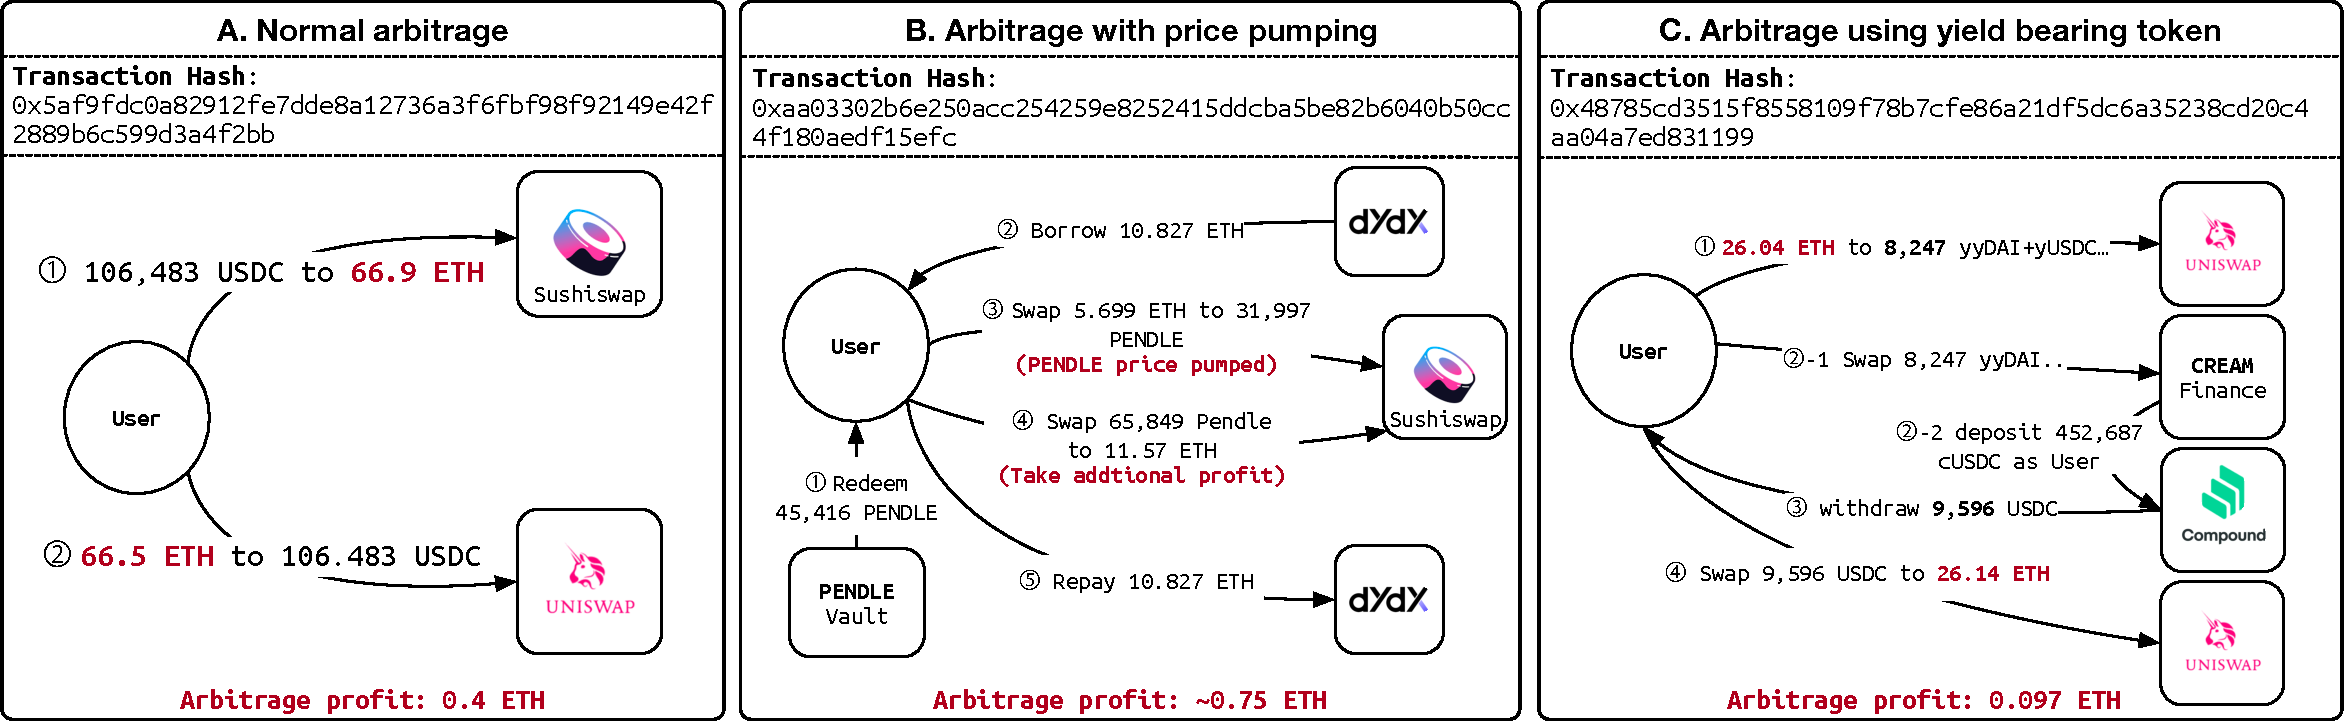
\includegraphics[width=\linewidth]{arbitrage_patterns.pdf}
  \caption{Representative evidence-trace patterns. Routine arbitrage is kept
  as a baseline, while manipulation and derivative paths require additional
  classification.}
  \label{fig:patterns}
\end{figure}

\subsection{Validation and Accuracy Evidence}
The strongest accuracy-style evidence currently carried into this public report
is the confirmed-incident validation from the paper-era regression suite:
\sys reconstructs all \numincidents curated incidents under its reconstruction
criteria. A prior scope-aware comparison table also reports DeFiRanger coverage
of 33/34 within its price-manipulation scope, while \sys covers 40/40 across
the broader incident set. This is validation evidence, not a full precision or
recall claim for the 14.2M-transaction IMC scale-out dataset.

\begin{table}[t]
\centering
\caption{Validation evidence retained for the public report.}
\label{tab:validation}
\begin{tabularx}{\linewidth}{l>{\raggedleft\arraybackslash}p{0.2\linewidth}X}
\toprule
Evaluation item & Result & Scope qualifier \\
\midrule
Confirmed-incident reconstruction & 40/40 & Curated public-incident set; verifies reconstruction criteria, not population prevalence. \\
DeFiRanger within-scope comparison & 33/34 & Price-manipulation specialization from the paper-era comparison. \\
Baseline arbitrage audit & 956 reviewed & IMC baseline separation; not a general false-positive-rate claim. \\
\bottomrule
\end{tabularx}
\end{table}

\section{Public Artifacts}
The public release is organized around reproducible artifacts rather than
paper-only claims.

\begin{table}[t]
\centering
\caption{Current public artifact status.}
\label{tab:artifacts}
\begin{tabularx}{\linewidth}{lX}
\toprule
Artifact & Status \\
\midrule
Source code & Present with public CLI; repository-wide TypeScript build cleanup remains open. \\
Technical report & This LaTeX/PDF report plus the Markdown planning report. \\
Example datasets & Synthetic schema sample and replayed bZx JSON. \\
Defect hash set & 219-hash public-looking subset with manifest; provenance review required before tag. \\
Non-baseline hash set & 1,386-hash broader candidate bundle with manifest; claim-scope review required before tag. \\
GitHub release path & Separate public repository at \url{https://github.com/appff/Evanesca_public}. \\
\bottomrule
\end{tabularx}
\end{table}

The artifact validator checks the example dataset schema and the public hash-set
counts:
\begin{verbatim}
npm run validate:public-artifacts
\end{verbatim}
The release also contains a smoke-test GitHub Actions workflow that installs
dependencies, validates artifacts, and checks the public CLI help path.

\section{Reward and Derivative Findings}
The paper-era investigation found two implementation-defect families that are
kept as public hash-set artifacts after provenance review: reward-distribution
manipulation and derivative-pricing/yield-bearing token deviation. Figure
\ref{fig:tend} illustrates a representative reward-distribution pattern. A
flash-loan-funded swap triggers reward behavior inside token logic and the
actor exits through a reverse path. The important point for \sys is not the
specific token, but that the reward effect and the profit-taking path occur
across contracts; a transaction-local SFG keeps those relations in one
evidence trace.

\begin{figure}[t]
  \centering
  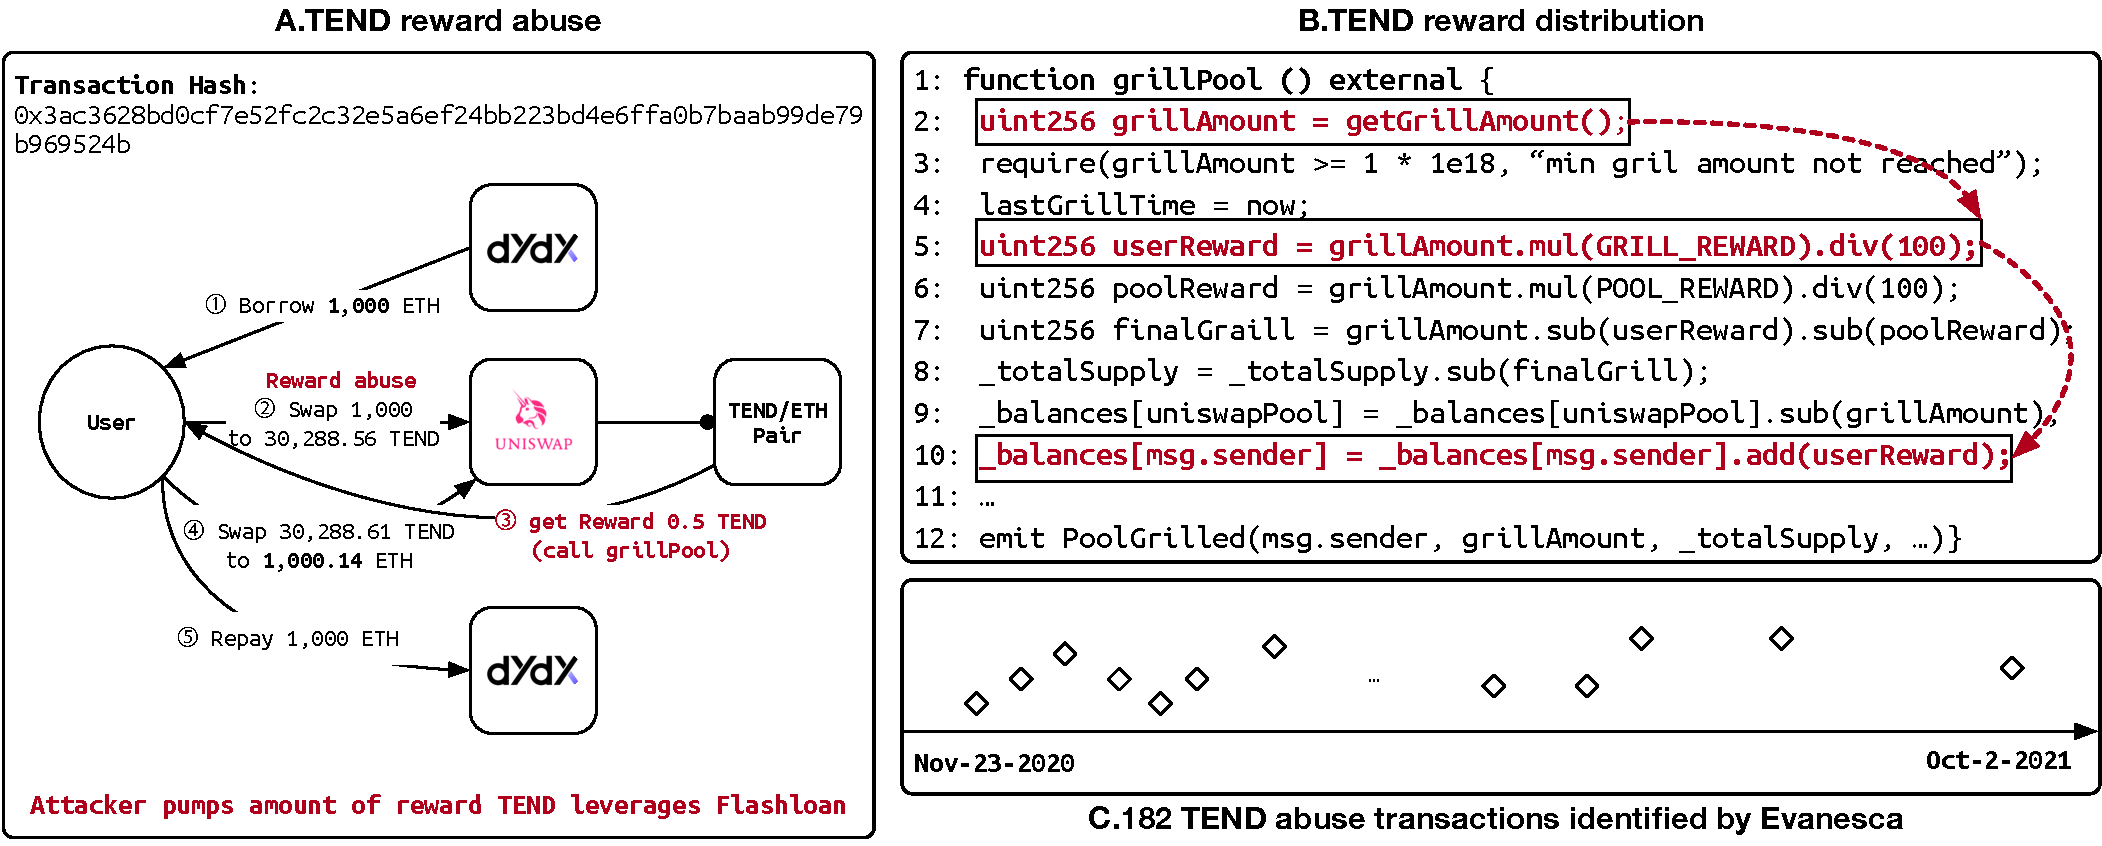
\includegraphics[width=\linewidth]{case_tend.pdf}
  \caption{Representative reward-distribution manipulation pattern from the
  paper-era artifact set.}
  \label{fig:tend}
\end{figure}

\section{Comparison With Prior Work}
\sys overlaps with prior DeFi attack-analysis and monitoring systems, but its
public release targets a different operational point.

\begin{table}[t]
\centering
\caption{Scope comparison.}
\label{tab:comparison}
\begin{tabularx}{\linewidth}{lXXX}
\toprule
System & Primary input & Main abstraction & Public release distinction \\
\midrule
DeFiRanger~\cite{wu2021defiranger} & Traces/events & Price-manipulation model & Strong baseline for known price manipulation. \\
BlockEye~\cite{wang2021blockeye} & On-chain events & Attack hunting/monitoring & Operational attack hunting. \\
DeFort~\cite{defort2024} & Transaction/state data & Price-manipulation analysis & Specialized automatic PM detection. \\
DeFiScope~\cite{zhong2025defiscope} & DeFi operations & PM reasoning workflow & Broad PM reasoning, LLM-assisted. \\
Forta/OZ~\cite{forta2023whitepaper,ozdefender} & Live deployment events & Rule alerts & Real-time operational monitoring. \\
\sys & Traces and semantic actions & SFG plus constraints & Reconstructs replayable candidate evidence across service classes. \\
\bottomrule
\end{tabularx}
\end{table}

This comparison should be sharpened before any future conference submission:
the public release can support case-by-case comparison, but it does not yet
provide a complete ensemble baseline or a precision/recall table against all
prior systems.

\section{Reproducibility}
A public claim should identify the code revision, configuration, dependency
lockfile, environment variables, input transaction hashes or dataset manifest,
command line, expected output, and limitations. The current minimum public
workflow is:
\begin{verbatim}
npm install
npm run analyze -- --help
npm run analyze -- --tx <transaction-hash> --chain ethereum \
  --out out/analysis.json --pretty
npm run validate:public-artifacts
\end{verbatim}

The bZx example has been replayed from a fresh public export without a local
\texttt{cache/} directory, using public RPC fallback providers. Population
artifacts still require external services such as Etherscan and Ethereum
archive/RPC access, as documented in the artifact manifests.

\section{Limitations and Release Gates}
\sys remains a research prototype. Current limitations include incomplete
adapter coverage, trace/RPC dependence, USD-normalization sensitivity, possible
false positives from unusual benign behavior, false negatives for unsupported
protocols or hidden state updates, and incomplete public labeling for the full
candidate population.

Before a stronger release tag or future conference submission, the project
should complete:
\begin{itemize}[leftmargin=*]
  \item repository-wide TypeScript build cleanup;
  \item dependency audit triage;
  \item implementation-synced constraint predicate documentation;
  \item public inclusion/exclusion criteria for confirmed incidents;
  \item threshold sensitivity analysis for \(\alpha\) and \(\beta\);
  \item human-labeling protocol for precision/recall claims;
  \item additional curated case-study JSON exports beyond bZx.
\end{itemize}

\section{Conclusion}
\sys exposes DeFi transactions as replayable financial-action evidence rather
than opaque alerts. The open-source release should therefore be judged by
whether its code, report, schema, artifacts, and examples let another researcher
inspect how a candidate was reconstructed. The current public package provides
that baseline: a source tree, technical report, evidence schema, replayed bZx
example, artifact manifests, and release checks. Future conference work can
build on this foundation by adding stronger correctness evaluation, prior-work
comparisons, and sensitivity analysis.

\bibliographystyle{plain}
\bibliography{evanesca-technical-report}

\end{document}
